\documentclass[11pt,a4paper]{article}
\usepackage[utf8]{inputenc}
\usepackage[german]{babel}
\usepackage{amsmath}
\usepackage{amsfonts}
\usepackage{subfig}
\usepackage{amssymb}
\usepackage{siunitx,physics}
\usepackage{mathtools}
\usepackage{graphicx}
%\usepackage{Here}
\usepackage[version=4]{mhchem}
\usepackage{url}
\usepackage{setspace}
\usepackage[left=2.5cm,right=2.5cm,top=2.5cm,bottom=2cm]{geometry}
[biblography=totocnumbered]
\usepackage{fancyhdr}
\usepackage{scrextend}
\usepackage{hyperref}
\pagenumbering{gobble}

\makeatletter
\newcommand\bigcdot{\mathpalette\bigcdot@{.5}}
\newcommand\bigcdot@[2]{\mathbin{\vcenter{\hbox{\scalebox{#2}{$\m@th#1\bullet$}}}}}
\makeatother

\makeatletter
%\renewcommand*\bib@heading{%
%  \subsection*{}%
%  \@mkboth{\refname}{\refname}}
%\makeatother
\numberwithin{equation}{section}
\numberwithin{figure}{section}

\renewcommand{\labelitemii}{\labelitemfont$\vartriangleright$}
\begin{document}\\
\begin{addmargin}[25pt]{0pt}
\begin{figure}[h]
    \centering
    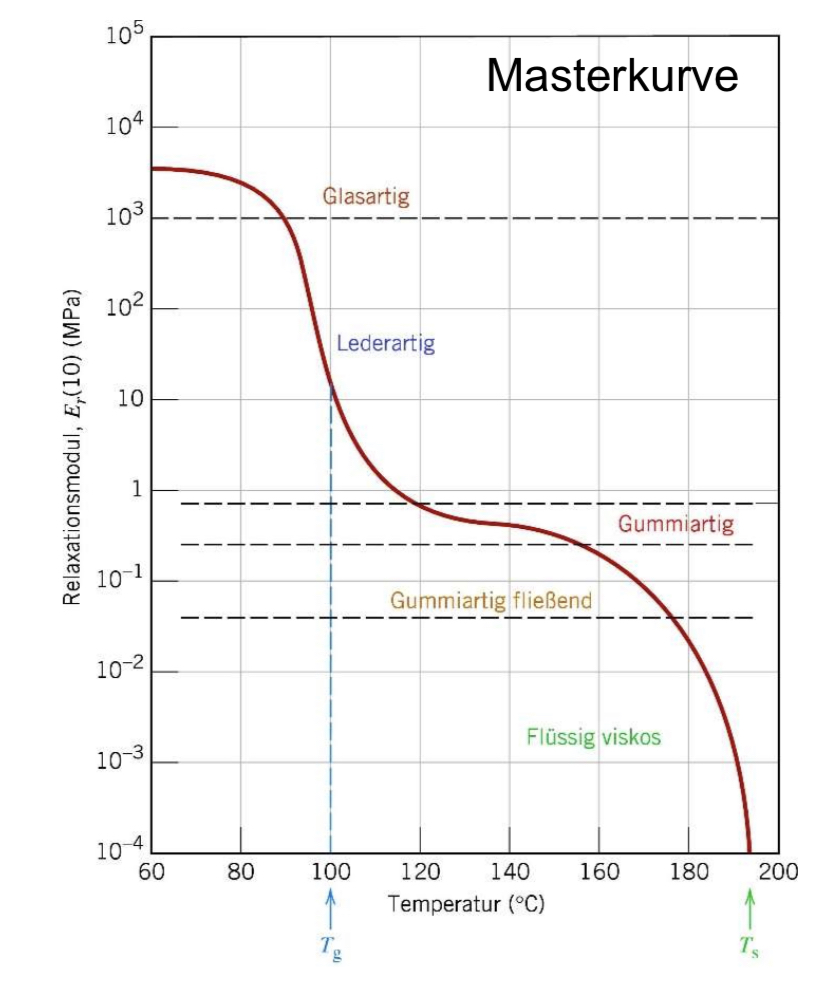
\includegraphics[width = 0.8\textwidth]{images/Materialwissenschaften/Masterkurve.jpeg}
    \caption{Beispiel einer Masterkurve mit den verschiedenen Bereichen für glasartig, gummiartig und fließend viskos}
    \label{fig:Masterkurve}
\end{figure}
Bei der Masterkurve wird der Relaxationsmodul gegen die Temperatur aufgetragen, dabei kann man dann ablesen im welchem Temperaturbereich das Material sich wie verhält. In Abbildung \ref{fig:Masterkurve} ist diese für amorphes Polystyrol beispielhaft dargestellt. Mit $T_g$ wird die Glasübergangstemperatur bezeichnet, das ist die Temperatur bei der das Verhalten des Glases von lederartig zu glasartig übergeht. $T_s$ ist die Schmelztemperatur, da geht der Relaxationsmodul gegen null.\\
\end{addmargin}

\end{document}